\documentclass[a4paper,12pt]{report}
\usepackage{a4wide}
\usepackage[brazil,english]{babel}
\usepackage[utf8]{inputenc}
\usepackage{hyperref}
\usepackage{doublespace}
\usepackage{fancyheadings}
\usepackage{abntcite}
\usepackage{graphics}
\usepackage{multirow}
\usepackage{epigraph}
\usepackage{url}
\usepackage{wrapfig}

\usepackage{url}
\usepackage{graphicx}
\usepackage{textcomp}
\usepackage{subfigure}
\usepackage[caixa=Mm,ordem=alf]{tabela-simbolos}
\usepackage{dsfont}
\def\citeopen{[}
\def\citeclose{]}

\newcommand{\figr}[1]{Figura~\ref{#1}}
\newcommand{\eqt}[1]{Eq.~(\ref{#1})}
\newcommand{\eqts}[2]{Eq.~(\ref{#1})~e~(\ref{#2})}
\newcommand{\eqtss}[3]{Eq.~(\ref{#1})~,~(\ref{#2})~e~(\ref{#3})}
\newcommand{\tab}[1]{Tabela~\ref{#1}}

%Comandos para se definir cabe�alhos nas p�ginas da disserta��o
\pagestyle{fancyplain}
\lhead[\fancyplain{}{\thepage}]{\fancyplain{}{\small\leftmark}}
\rhead[\fancyplain{}{\small\rightmark}]{\fancyplain{}{\thepage}}
\cfoot{\fancyplain{\thepage}{}}

%Configuração para numeração de subsubseções
\setcounter{secnumdepth}{3}
%Instancia do contador que ser� usado como refer�ncia na monografia
\newcounter{mypage}
\DeclareGraphicsExtensions{.jpg, .pdf, .mps, .png}

\begin{document}
\stepcounter{mypage}

\thispagestyle{empty}

\begin{spacing}{1.0}

\begin{center}
\begin{figure}[!htb]
    
\includegraphics[scale=0.3, bb=0 0 1500 400]{ucam.png}
\end{figure}
\end{center}

\vspace {2 cm}
\begin{center}
\begin{normalsize}
\uppercase{
Gabriel Manhães Monnerat
}
\end{normalsize}
\end{center}
\vspace {2 cm}
\begin{spacing}{1.5}
\begin{center}
\begin{Large}
{\bf \uppercase{Ferramenta para manipulação de documentos em larga escala}
}
\end{Large}

\end{center}
\end{spacing}

\vspace {5 cm}

\begin{center}

\begin{large}
Campos dos Goytacazes - RJ \\[0.2 cm]
Junho - 2010
\end{large}
\end{center}

\end{spacing}
\newpage
\stepcounter{mypage}

\thispagestyle{empty}

\begin{spacing}{1.0}

\begin{center}
\begin{large}
\uppercase{
Gabriel Manhães Monnerat} \\[0.2 cm]
\end{large}
\end{center}

\vspace {5 cm}

\begin{spacing}{1.5}
\begin{center}
\begin{Large}
{\bf \uppercase{Ferramenta para manipulação de documentos em larga escala}}
\end{Large}
\end{center}
\end{spacing}

\vspace {2 cm}

\begin{flushright}
\begin{minipage}[t]{8.5 cm}
Monografia apresentada à Universidade Candido Mendes como requisito obrigatório para a obtenção do grau de Bacharel em Ciência da Computação.
\end{minipage}
\end{flushright}

\vspace {1.5 cm}

\begin{center}
\begin{large}
ORIENTADOR: Prof. D.Sc. Dalessandro Soares Vianna\\[0.2 cm]
\end{large}
\end{center}

\vspace {1.5 cm}

\begin{center}
\begin{large}
Campos dos Goytacazes - RJ\\[0.2 cm]
Junho - 2010
\end{large}
\end{center}

\end{spacing}
\newpage


\stepcounter{mypage}

\thispagestyle{empty}

\begin{spacing}{1.0}

\begin{center}
\end{center}

\vspace {1.0 cm}

\begin{center}
\begin{Large}
{\bf \uppercase{Ferramenta para manipulação de documentos em larga escala}
} \\[0.2 cm]
\end{Large}
\end{center}

\vspace {1.0 cm}

\begin{flushright}
\begin{minipage}[t]{8.5 cm}
Monografia apresentada à Universidade Candido Mendes como requisito obrigatório para a obtenção do grau de Bacharel em Ciência da Computação.
\end{minipage}
\end{flushright}

\vspace {1.5 cm}

\begin{center}
\begin{large}
Aprovada em \_\_\_\_ de \_\_\_\_\_\_\_\_\_\_\_\_ de 2010. \\[0.2 cm]
\end{large}
\end{center}

\vspace {1.5 cm}

\begin{center}
\begin{large}
BANCA EXAMINADORA \\[0.2 cm]
\end{large}
\end{center}

\vspace {1 cm}

\begin{center}
\line(1,0){300}\\ 
Prof. Dalessandro Soares Vianna - Orientador \\
Universidade Federal Fluminense\\

\end{center}

\vspace {1.0 cm}

\begin{center}
\line(1,0){300}\\ 
Prof. Fernando Carvalho\\
Instituto Federal de Educacao, Ciência e Tecnologia Fluminense / Campus Bom Jesus
\end{center}

\vspace {1.0 cm}

\begin{center}
\line(1,0){300}\\
Prof Fábio Duncan de Souza\\
Instituto Federal de Educacao, Ciência e Tecnologia Fluminense / Campus Campos\\
\end{center}

\end{spacing}
\newpage

\stepcounter{mypage}

\thispagestyle{empty}

\

\vfill

\begin{flushright}
\textit{Dedico este trabalho a meus pais, irmão, namorada e amigos por todo apoio e compreensão prestado durante essa importante fase da minha vida.}
\vspace*{1cm}

\end{flushright}

\vspace*{1cm}

\clearpage

\stepcounter{mypage}
%Include dos agradecimentos
\chapter*{Agradecimentos}
\thispagestyle{empty}
Primeiramente gostaria de agraceder a meus pais e namorada que me apoiaram e estiveram do meu lado em todos os momentos.

Agradeço ao Nucleo de Pesquisa em Sistema de Informaçao(NSI) por me proporcionar recursos financeiros e materiais para o desenvolvimento deste trabalho.

Agradeço a Dalessandro que sempre esteve disposto a ajudar durante o desenvolvimento deste trabalho. 

Agradeço também a Rogério Atem, Fabio Duncan e William da Silva Vianna que sempre buscaram o melhor para minha vida profissional quanto para todos os seus bolsistas e alunos. Em especial gostaria de agradecer a Herman Caldara e Rafael Gonçalves que me ajudaram e se empenharam no desenvolvimento deste trabalho como se este fosse o trabalho deles.
 
\thispagestyle{empty} 

\stepcounter{mypage}

% \null
\vfill
\epigraph{Para ter sucesso basta ter fé.}{Gabriel Monnerat}
% \stepcounter{mypage}

\renewcommand{\baselinestretch}{1.3}
\pagenumbering{roman}

\setlength{\voffset}{0.0in}

%Atribui ao contador page (default do latex, que é usado por todo o documento)
%o valor do contador é mypage
\setcounter{page}{\value{mypage}}
%Espaçamento das páginas
\begin{spacing}{1.5}
%Include do resumo
\chapter*{Resumo}
\label{resumo}
Este trabalho desenvolve uma ferramenta que tem o objetivo de substituir uma já existente que com o uso excessivo e prolongado mostrou problemas graves de escalabilidade e confiabilidade, sendo necessário a criação de uma nova ferramenta para além de correção dos problemas, realizar uma busca por padrões mais consolidados e atingir uma estrutura mais flexível. Neste trabalho são apresentados conceitos básicos que foram utilizados para o desenvolvimento desta ferramenta e, além disso, junto com a descrição da ferramenta foram discutidas soluções para os problemas já conhecidos. Para validação da ferramenta desenvolvida,  foi aplicado em um estudo de caso simples para desmonstrar o uso similar ao de produção.

\vspace{0.5cm}
PALAVRAS-CHAVE: Internet - Serviço Web - Desenvolvimento de Software - Escalabilidade
\end{spacing}

\selectlanguage{brazil}

\begin{spacing}{1.0}
\listoffigures
\listoftables
\tableofcontents
\end{spacing}

\clearpage
\setcounter{mypage}{\value{page}}
\clearpage
\pagenumbering{arabic}

%Includes da monografia propriamente dita
\begin{spacing}{1.5}
\setcounter{page}{\value{mypage}}
\chapter{Introdução}
A Internet, uma das grandes revoluções tecnológicas da comunicação dos últimos dez anos, deve essa popularidade ao avanço na tecnologia Web, que popularizou uma interface gráfica intuitiva baseada em \textit{hiperlinks}, possibilitando a fácil utilização dos serviços disponibilizados via internet. O crescente volume de computadores conectados a rede altera profundamente o modo de desenvolvimento dos aplicativos, obrigando corporações a introduzirem novas tecnologias que suportem a grande demanda. Logo, com o crescimento tanto de usuários quanto de aplicações via rede de computadores, novas dificuldades surgiram com a extensão das aplicações, como maior complexidade de manutenção, a dificuldade de inserir novas funcionalidades e a curva de aprendizado acentuada aos desenvolvedores. Visando minimizar estas dificuldades, surge a necessidade de serviços descentralizados, mais simples e com uma confiança maior para desenvolvimento de softwares em larga escala.

Com a descentralização das informações, o desenvolvimento de sistemas simples e escaláveis fez com que surgissem cada vez mais serviços Web que tivessem somente uma responsabilidade e pudessem se comunicar com outros aplicativos via internet ou intranet. Em resumo, serviços simples, de fácil manutenção e extensão, proporcionam o aumento da perfomace e escalabilidade, eliminando o uso de um serviço único com todo volume de informações para serem processadas constantemente.

A iniciativa entre a empresa francesa Nexedi SA(empresa situada em Lille, França) e o NSI(Núcleo de pesquisa em Sistema de Informação) do Instituto Federal Fluminense-Campos de desenvolverem uma ferramenta Web de código aberto que subsitui-se uma já existente, chamada OpenOffice.org Daemon (oood), desenvolvida originalmente pela Nexedi SA, é um exemplo da necessidade do uso de novas tecnologias para suportar novas demandas e requisitos.

A primeira versão do oood foi desenvolvida em 2006 pela Nexedi com o objetivo inicial de converter documentos do tipo Office. A partir do uso prolongado em ambientes de produção foram identificados erros ou tratamentos inadequados de exceções que ocasionaram problemas como: perda de requisições, \textit{deadlock} no OpenOffice.org e em processos, \textit{memory leak}, entre outros. Logo, surgiu a necessidade de corrigir o serviço para torná-lo mais estável, com um bom desempenho e escalável em forma de cluster. A análise preliminar do oood determinou que seria inviável a manutenção do mesmo, pois havia demanda por novos requisitos e a necessidade de corrigir os problemas mencionados acima.

Com a necessidade da correção dos problemas identificados e o uso de resursos mais atuais e estáveis, surge a motivação para o desenvolvimento de uma nova ferramenta que tivesse como funcionalidades básicas converter documentos para a base ODF (\textit{Open Document Format}), exportar documentos para outras extensões, adicionar e extrair metadados de um documento nos formatos suportados pelo OpenOffice.org. Outros fatores que também influenciaram na iniciativa de uma nova ferramenta foi a busca por uma estrutura mais flexível, de fácil manutenção, extensível e escalável.

Portanto, este trabalho tem como objetivo desenvolver uma ferramenta Web que utilize de recursos computacionais para manipulação de documentos, de forma que seja possível extrair e adicionar informações e fazer conversões destes documentos para qualquer formato suportado pelo Openoffice.org. Além disso, apresentar soluções para os problemas identificados, tais como \textit{deadlock} no OpenOffice.org, perda de requisições e falta de escalabilidade.

No segundo capítulo são apresentados conceitos básicos para melhor entendimento das tecnologias e padrões utilizados durante o trabalho. No terceiro capítulo, é explicado separadamente cada componente desenvolvido com o intuito de apresentar no quarto capítulo estudos de casos descrevendo em detalhes como a junção destes componentes formam um serviço Web e o uso deste em um ambiente similiar ao de produção.

Por fim, o quinto capítulo apresenta os resultados obtidos com o estudo de casos e a conclusão obtida a partir do desenvolvimento desta aplicação.
\chapter{Conceitos básicos}
\label{cap2}
Nas seções seguintes serão apresentados conceitos, tecnologias, padrões e ferramentas que são essenciais para o entendimento deste trabalho.

\section{\textit{OpenDocument Format}}
O \textit{OpenDocument Format}(ODF), forma abreviada de \textit{OASIS OpenDocument Format for Office Applications}, é um conjunto de formatos de arquivos para aplicações de escritório(edição de texto, planilhas, apresentações de slides, banco de dados, manipulação de imagens, entre outros) desenvolvido com a proposta de oferecer um padrão aberto que pode ser adotado por qualquer pessoa ou instituição. 

Esse padrão foi desenvolvido pelo consórcio OASIS e é baseado no formato XML. O acesso a este padrão é público, o que possibilita a implementação em qualquer sistema, seja ele de código aberto ou não. Segundo \cite{ronaldo}, a intenção do formato ODF é prover uma alternativa aos formatos proprietários de documentação, para que não fiquem aprisionados a um único fornecedor.

Nas subseções seguintes será apresentada a estrutura deste formato e os formatos de documentos para cada tipo de documento.

\subsection{Estrutura de um \textit{OpenDocument}}

Por ser em código aberto, é possível ter acesso a todos os dados de um documento, pois são arquivo compactados e utilizam arquivos XML para estruturar seus dados \cite{oasis}. Então, quando um documento em ODF é criado, um conjunto de arquivos e pastas o constitui. Os principais são:
\begin{itemize}
 \item mimetype - Arquivo de linha única com o \textit{mimetype} do documento;
 \item content.xml - Arquivo que armazena o conteúdo do documento criado pelo usuário;
 \item meta.xml - Armazena os "metadados" do documento, ou seja, informações como autor, data de modificação, quantidade de palavras, etc;
 \item styles.xml - Contém estilos para o documento, por exemplo, formatações específicas para parágrafos e listas;
 \item Pictures - Pasta que armazena as imagens do documento;
\end{itemize}

\subsection{Formatos \textit{OpenDocument}}
Para todo tipo de documento, como por exemplo texto, existe um formato base para este tipo. Os formatos para cada tipo são apresentados na Tabela \ref{tab:tabela1}.
\begin{table}[htb] 
   \centering 
   \large
   \setlength{\arrayrulewidth}{2\arrayrulewidth}  % espessura da  linha
   \setlength{\belowcaptionskip}{10pt}  % espaço entre caption e tabela
   \caption{\it Tabelas de formatos \textit{OpenDocument}}
   \begin{tabular}{|c|c|} % c=center, l=left, r=right 
      \hline
      odt & Documento de Texto \\
      \hline 
      ods & Panilha Eletrônica \\
      \hline
      odp & Documento de Apresentação \\
      \hline
      odg & Desenho Vetorial \\
      \hline
      odf & Equações \\
      \hline
      odb & Banco de Dados \\
      \hline
      odj & Documento Mestre \\
      \hline
   \end{tabular}
   \label{tab:tabela1}
\end{table}

Na seção seguinte será apresentado um software de manipulação de documentos que têm como padrão o ODF.

\section{OpenOffice.org}
Inicialmente o OpenOffice.org era chamado de StarOffice. A Sun MicroSystems comprou este software na versão 5.1, em 1999, da empresa alemã StarDivison. Em agosto de 1999, a Sun disponibilizou gratuitamente a versão 5.2 do StarOffice e em meados de 2000 anunciou a liberação do código fonte para \textit{download} sob as licenças \textit{Lesser General Public License}(LGPL) e \textit{Sun Industry Standards Source License}(SISSL) com o intuito de criar uma alternativa de baixo custo, código aberto e de alta qualidade. LGPL e SISSL impõem que o código aberto desenvolvido esteja disponível em forma de biblioteca, mas não exige que o mesmo seja aplicado a outros softwares que empreguem seu código \cite{wiki:oo.org}. No mesmo ano da liberação da versão 5.2 do StarOffice, o novo projeto recebe o nome de OpenOffice.org e no Brasil de BrOffice.org.

Segundo \cite{ronaldo}, OpenOffice.org é uma suíte de aplicativos multiplataforma, sendo distribuída para sistemas operacionais como Linux, Microsoft Windows, Solaris e Mac OS X. A suíte usa os formatos ODF e é compatível com formatos da Microsoff Office. No caso de documentos que não estão no formato ODF, estes arquivos são convertidos para uma extensão de mesmo tipo que seja ODF. O OpenOffice.org divide estas extensões em tipos, ou seja, cada documento tem o seu próprio tipo e só pode ser convertido para outra extensão que faça parte do seu grupo de tipos. As extensões nas suítes são dividas em 5 tipos onde cada tipo tem a sua extensão padrão. Por exemplo, um documento do tipo texto é convertido para o formato ODT quando carregado no aplicativo OpenOffice.org. Com essa padronização, documentos criados e suportados pelo aplicativo são compatíveis com instalações do mesmo software em outros sistemas operacionais.

A seção seguinte apresenta o UNO que é um mecanismo utilizado para comunicação entre linguagens de programação e o OpenOffice.org.

\section{UNO}
UNO ou \textit{Universal Network Object} é um modelo de componentes do OpenOffice.org, que oferece interoperabilidade entre linguagens de programação e o modelo de objetos do OpenOffice.org, ou seja, componentes UNO podem ser implementados e acessados a partir de uma linguagem de programação \cite{uno_page}. Estes componentes têm recursos idênticos de uma aplicação OpenOffice.org aberta em um sistema operacional, como por exemplo abrir um documento em um formato específico e salvá-lo em outro formato suportável.

Para entender melhor como é o funcionamento do UNO, que tem uma idéia diferente de programação comparada à programação tradicional, é necessário distinguir entre especificação e implementação. Em aplicações normais, as especificações são declaradas em documentos na linguagem natural. Em contrapartida, UNO declara seus métodos e propriedades em uma \textit{Application Programming Interface}(API) chamada IDL. 

IDL é uma linguagem de computador utilizada para descrever interfaces de componentes de softwares. Esta linguagem de programação é independente, com isso possibilita a comunicação de linguagens diferentes. Ou seja, na IDL não existe nenhuma implementação de código, existe somente a declaração e descrição dos métodos. A implementação é realizada na linguagem de programação que possui biblioteca para acessar os recursos do UNO, como demonstra a Figura \ref{fig:uno_picture} a separação da especifição e linguagens que possuem pontes para se comunicar com o UNO.

Com a IDL tem-se a fácil comunicação entre uma linguagem de programação e o UNO, seja intranet ou internet. Quando se está com um aplicativo da suíte OpenOffice.org aberto, tem-se por trás de todo os recursos uma utilização constante de componentes UNO de acordo com o uso do aplicativo. Lembrando que, mesmo o UNO sendo usado internamente, é através de uma linguagem de programação que é feita a comunicação entre OpenOffice.org e UNO.

\begin{figure}[ht]
\centering
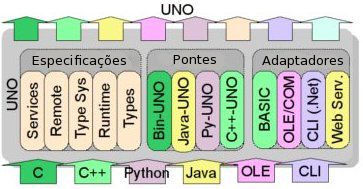
\includegraphics[scale=0.55,bb=0 0 510 180]{Uno-Arc.png}
\caption{Arquitetura do UNO. Adaptado de: \cite{uno_page}.}
\label{fig:uno_picture}
\end{figure}

A sessão seguinte apresenta uma biblioteca implementada em Python para utilizar o UNO nesta linguagem.

\subsection{PyUNO}
A biblioteca PyUNO permite que toda a API do OpenOffice.org seja utilizada na linguagem de programação Python de formas diferentes, como por exemplo utilizar \textit{scripts} executáveis em Python e através do \textit{framework} de \textit{scripts} do OpenOffice.org. A biblioteca não contém métodos que acessam o UNO, visto que toda implementação do UNO é carregada no Python \cite{pyuno_page}. Isto faz com que todo uso dos componentes seja no Python, toda especificação esteja na IDL e toda implementação no próprio UNO.

A subseções seguintes apresentam formas de utilização desta biblioteca.

\subsubsection{Python \textit{Scripts}}
\textit{Scripts} em Python são executáveis que se conectam ao OpenOffice.org utilizando o UNO. De todas maneiras possíveis, a utilização de \textit{scripts} é a forma mais lenta de uso, pois toda transferência é feita via conexão de rede. Como são implementados em Python, os \textit{scripts} são independentes do OpenOffice.org. A Figura \ref{pyuno.png} mostra como é executado um Python \textit{script}.
\begin{figure}[ht]
\centering
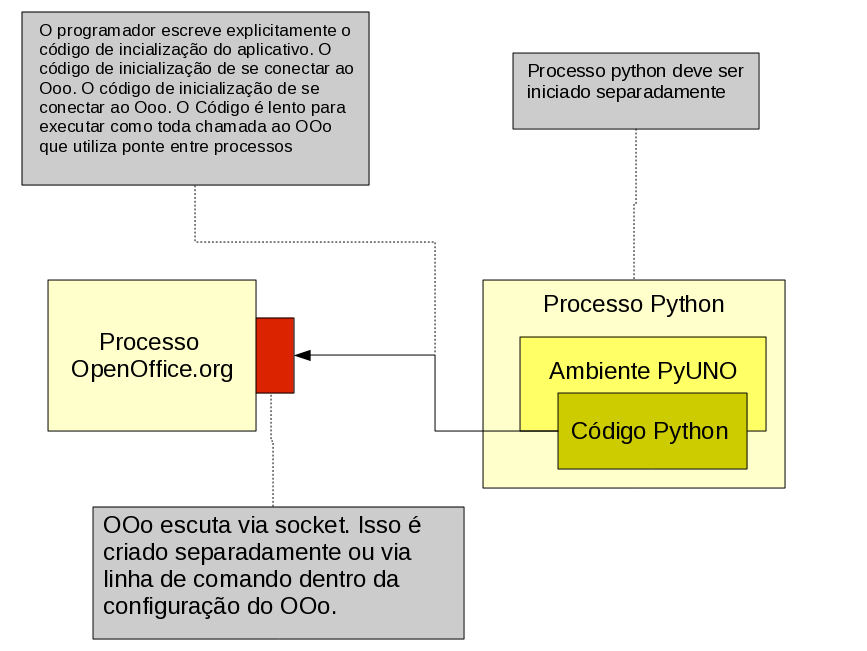
\includegraphics[scale=0.45,bb=0 0 634 460]{pyuno2.png}
\caption{\textit{Scripts} Python Utilizando PyUno. Adaptado de: \cite{web:uno}.}
\label{pyuno.png}
\end{figure}

Analisando a Figura \ref{pyuno.png} percebe-se que parte do código em Python é executado dentro do ambiente do PyUNO. Estes códigos são chamadas à API do UNO para criação dos componentes e a outra parte do código faz uso ou não destes objetos. Um exemplo de uso dos componentes do UNO é a criação do objeto que faz conexão ao processo OpenOffice.org.

\subsubsection{\textit{Script} Python como componente UNO}

Desta forma, os Python \textit{scripts} são implementados para serem inseridos dentro do OpenOffice.org, com isso há um ganho de desempenho pois não há necessidade de fazer conexão entre o processo OpenOffice.org e o Python \textit{script}. A Figura \ref{mode_component.png} mostra como o componente trabalha dentro de um processo OpenOffice.org.

\begin{figure}[ht]
  \centering
  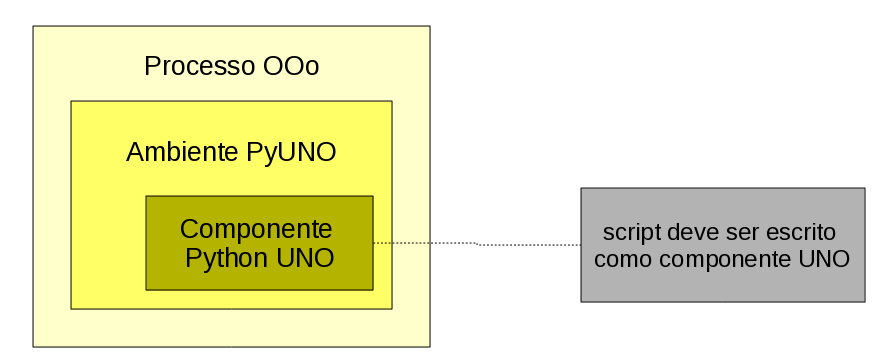
\includegraphics[scale=0.41,bb=0 0 574 257]{mode_component2.png}
  \caption{\textit{Scripts} Python como componente UNO. Adaptado de: \cite{web:uno}.}
\label{mode_component.png}
\end{figure}

\section{XML}

Segundo, \cite{xml_dummies}, XML é uma linguagem de marcação que utiliza \textit{tags} para rotular, categorizar e organizar as informações de maneira específica. A marcação descreve o documento ou a organização do mesmo. O conteúdo, como textos, imagens e dados, são partes do código que as \textit{tags} de marcação contêm. Além disso, o XML não está limitado a um conjunto especifíco de marcações, estas podem ser criadas para atender às necessidades, como exemplo a Figura \ref{xml.png} demonstra a criação de novas \textit{tags} de marcação para representar alunos.

\begin{figure}[ht]
\centering
\begin{center}
   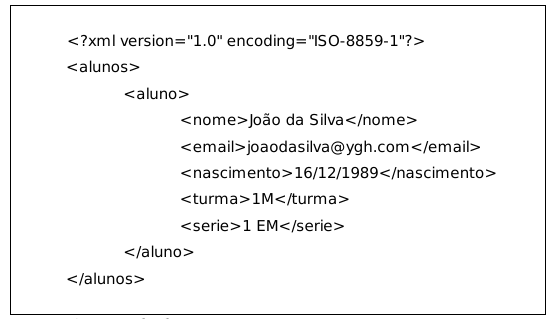
\includegraphics[scale=0.55,bb=0 0 450 236]{xml.png}
\end{center}
\caption{Exemplo de Arquivo XML. Fonte: \cite{ronaldo}.}
\label{xml.png}
\end{figure}

Pode ser notado na Figura \ref{xml.png}, a própria estrutura e declaração das \textit{tags} do XML declaram o conteúdo do documento, facilitando a leitura dos dados através de outras linguagens de programação.

\section{WSGI}
\label{wsgi}
Historicamente o \textit{Web Service Gateway Interface}(WSGI) foi proposto em 2003 por Philip J. Eby e programadores Python. Esta proposta, segundo \cite{wsgi:website}, tinha objetivo de criar um caminho fácil de integrar diferentes aplicações Web e obter uma única aplicação final.

Python possui atualmente uma variedade de \textit{frameworks} para construção de aplicações Web, tais como Zope, Django, Twisted Web, entre outros. Essa variedade tem um lado positivo onde é possível escolher um \textit{framework} que atenda melhor as necessidades atuais do desenvolvedor. Mas por outro lado, a escolha do \textit{framework Web} irá limitar a seleção de serviços Web utilizáveis, e vice-versa.

Em contrapartida, embora a linguagem de programação Java tenha também uma variedade de \textit{frameworks} disponíveis para construção de aplicações Web, esta tem a Java Servlet API que torna possível que aplicações desenvolvidas em qualquer \textit{framework Web} Java rode em qualquer servidor Web que suporta a API do \textit{servlet}.

Com a possibilidade de qualquer servidor Web rodar qualquer aplicação Web, tem-se o desenvolvimento independente da escolha do servidor Web. Além disso, deixa livre os desenvolvedores para escolherem o que melhor os atendam e se concentrar em sua área de especialização, deixando para outro desenvolvedor a responsabilidade de escolher qual servidor Web utilizar.

Em suma, esta proposta tenta resgatar a independência de aplicações e servidores Web como o Java Servlet API, para que facilite a escolha da tecnologia a ser utilizada tanto no desenvolvimento da aplicação quanto na ferramenta servidora.

\section{\textit{Web Service}}

Existem diferentes maneiras de definir um \textit{Web Service}. \citeonline{w3c}  define \textit{Web Service} como:
\begin{quote}
\textit{Um software projetado para suportar interações interoperáveis entre máquinas sobre uma rede. Tem uma interface descrita em um formato processável por máquina(especificamente WSDL). Outros sistemas interagem com este serviço Web de uma maneira prescrita usando mensagens SOAP, tipicamente transmitida usando HTTP com serialização XML em conjunto com outras normas relacionadas à Web.}
\end{quote}

\textit{Simple Object Acess Protocol}(SOAP), citado por \cite{w3c}, é um protocolo baseado em XML para troca de informações entre computadores, tendo seu foco principal a chamada de procedimentos remotos transportados via HTTP \cite{ethan}. Portanto, permitem que aplicativos cliente possam facilmente conectar-se a serviços remotos e invocar metódos. 

\textit{Web Service Description Language}(WSDL), também citado por \cite{w3c}, é um formato XML para descrever serviços de rede como um conjunto de parâmetros operacionais sobre as mensagens que contenham qualquer informação ou documento orientado para processo de orientação. As operações e mensagens são descritas abstratamente e estão ligado a um protocolo de rede concreto e formato de mensagem para definir um ponto de extremidade \cite{wsdl}.

Em outras palavras, é uma solução utilizada na integração de sistemas e na comunicação entre aplicações de diferentes arquiteturas \cite{book:webservice}, como demonstra a Figura \ref{imagem:webservice}.

\begin{figure}[ht]
 \centering
 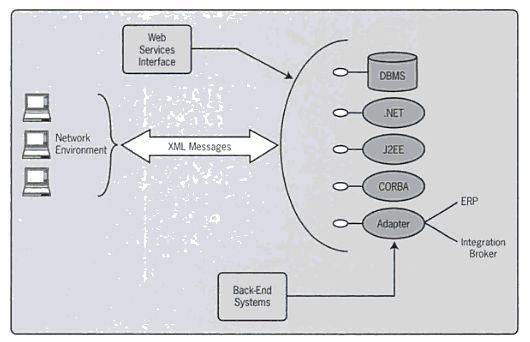
\includegraphics[scale=0.80,bb=0 0 450 250]{webservice_exemplo.png}
 \caption{Serviço Web com sistemas internos de plataformas diferentes, Adaptado de: \cite{webservice_foto}.}
\label{imagem:webservice}
\end{figure}

Note que na Figura \ref{imagem:webservice}, os clientes enxergam a aplicação como um sistema único e utilizam o mesmo protocolo de comunicação. Com isso, há uma independência tanto do cliente quanto do servidor, permitindo que estes exerçam o seu papel da melhor maneira possível.

Segundo \cite{ethan} e \cite{naveen}, existem três papéis principais dentro da arquitetura de serviços Web:
\begin{itemize}
 \item Prestador de Serviço - Fornece os serviços através da Web e responde os pedidos dos consumidores;
 \item Consumidor de Serviço - Utiliza uma rede existente através da abertura de uma conexão de rede e envia uma solicitação em XML. Em serviços Web baseados em SOAP, o prestador de serviço publica o contrato(WSDL) do serviço através da internet e o consumidor pode acessá-lo diretamente ou buscar o registro de serviço;
 \item Registro de Serviço - Diretório lógico centralizado de serviços onde os desenvolvedores podem publicar ou encontrar novos serviços já existentes, portanto, serve como uma agência centralizada para as empresas e seus serviços.
\end{itemize}

Com esta arquitetura flexível, um \textit{Web Service} pode ser um caminho para expansão dos negócios de uma empresa, com o objetivo de aumentar a eficiência do processo de negócio e sua experiência com o cliente, já que este não está limitado à automatização dos processos \cite{singh}. Além disso, pode simplificar as interações com serviços externos, tais como validação do cartão de crédito ou compra com o mesmo. Como resultado, são oferecidos aos clientes uma experiência enriquecida, com mais opções de escolha e mais flexibilidade. 

Com isso, cada \textit{Web service} é responsável por um processo, ou seja, cada aplicação tem a sua responsabilidade. Por exemplo um sistema que controla usuário e senha em um caixa eletrônico, é responsável somente autenticar usuários. Logo, tendo poucas atribuições ao serviço faz-se o uso do mesmo com mais rapidez e clareza.

\section{XML-RPC}
Segundo \cite{laurent}, XML-RPC é um dos métodos mais simples de serviços Web, e que torna fácil computadores chamarem procedimentos de outros computadores. Este método permite que programas façam chamadas de função ou procedimento em uma rede utilizando o protocolo \textit{Hypertext Transfer Protocol}(HTTP) para transferir informações de um computador cliente a um computador servidor. É utilizado a linguagem XML tanto para fazer requisições pelo cliente quanto para responder a ele. A Figura \ref{xmlrpc.jpg} apresenta como é a comunicação e a transferência das informações entre cliente e servidor.

\begin{figure}[ht]
 \centering
 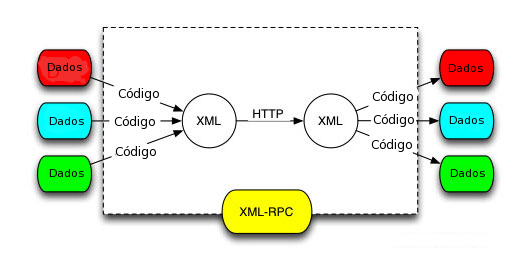
\includegraphics[scale=0.50,bb=0 0 550 250]{xmlrpc.jpg}
 \caption{Troca de mensagens utilizando XML-RPC, Adaptado de Fonte: \cite{web:xmlrpc}.}
\label{xmlrpc.jpg}
\end{figure}

Em uma arquitetura cliente-servidor, todos procedimentos são requisitados pelo cliente e executados pelo servidor. Para que isto seja possível utiliza-se uma das tecnologias de comunicação entre processos, a \textit{Remote Procedure Call}(RPC). RPC permite a um programa de computador chamar um procedimento no mesmo computador ou em outro conectado por uma rede. No caso do XML-RPC todas as chamadas são feitas através de uma rede de computadores mas para o RPC não existe diferença entre o procedimento estar na mesma máquina ou em outro computador.

\section{ERP}
\textit{Enteprise Resource Planning}(ERP) é um sistema de informação usado para gerenciar os recursos internos e externos de uma corporação \cite{wiki:erp}. Sua arquitetura tem como objetivo a facilidade de gestão do fluxo de informações, sendo este gerado pela integração dos dados e processos de vários ou mesmo da totalidade dos departamentos da organização num único sistema. Esta integração pode ser efetuada ao nível departamental ou funcional (sistemas finanças, marketing, comercial, pessoal, produção, etc.) ou ao nível processual(sistema de tratamento de encomendas, sistema de informação de gestão, sistema de apoio à decisão, etc.) \cite{557044}. 

Resumidamente, segundo \cite{557044}, ERP é uma tecnologia de suporte de software que forma um núcleo de processamento de transações, tendo sua aplicação em várias áreas.

\section{ERP5}

Para \cite{artigo:rogerio}, o ERP5 é um ERP de código aberto que visa oferecer uma solução de alta tecnologia e baixo custo, sendo desenvolvida pela Nexedi, criadora do software, e instituições de pesquisa de países da Europa e do Brasil. Este software é desenvolvido na plataforma Zope, escrito na linguagem de programação Python. O Zope é um servidor de aplicações Web de código aberto desenvolvido em Python \cite{python_zope} que oferece um banco de dados orientado a objeto(ZODB) e um máquina de estado(DC Workflow). Com isso, além de utilizar os recursos oferecidos pela plataforma, o ERP5 incorpora a sicronização entre diferentes bancos de dados orientado a objeto e um mecanismo de mapeamento de banco de dados relacional que indexa atributos de cada objeto em um banco de dados relacional \cite{handbook}.

\subsection{\textit{Business Templates}}
\textit{Business Templates} é a utilização de componentes existentes no ERP5 para adicionar novas funcionalidades ao núcleo do ERP5. Em outras palavras, a partir da reutilização dos recursos, campos e \textit{scripts}, é possível criar modelos de negócio utilizando componentes já existentes \cite{beautiful}.

\section{Buildout}

Buildout é uma ferramenta, desenvolvida em Python, que fornece suporte para criação de aplicações, seja ela desenvolvida em Python ou em outra linguagem de programação \cite{jim}. Entre vários mecanismos de criação e instalação de aplicações que o Buildout utiliza, os \textit{recipes} são os mais utilizados. \textit{Recipes} são \textit{scripts} Python que executam algum procedimento específico e possuem todas as informações do Buildout que está executando-o. A Figura \ref{buildout.png} é um exemplo de um arquivo de configuração do Buildout. 

\begin{figure}[ht]
 \centering
 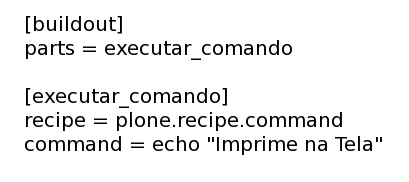
\includegraphics[scale=0.50,bb=0 0 550 250]{buildout.png}
 \caption{Arquivo de configuração do Buildout.}
\label{buildout.png}
\end{figure}

Na organização do arquivo de configuração, existem dois atributos importantes no buildout que são: \textit{parts}, \textit{recipe}. O \textit{parts} é utilizado para declarar qual procedimento será chamado. Dentro da declaração do procedimento tem o atributo \textit{recipe} que por sua vez é o caminho do script que executará todo procedimento. Por fim, na Figura \ref{buildout.png} temos além da declaração dos atributos essenciais, temos um atributo \textit{command}. Este atributo será utilizado pelo \textit{recipe} que foi implementado para executar o que estiver dentro do \textit{command}.

Em suma, o Buildout é extremamente flexível e simples para criação de ambientes de desenvolvimento específicos e enxutos.
 
\section{Subversion}

Segundo \cite{975530}, Subversion é um sistema de controle de versão de código aberto. Sistemas de controle de versão são utilizados em ambientes de desenvolvimento de software para controlar diferentes versões do código-fonte e possibilitar o trabalho em equipe. Para que isto ocorra, é fornecido pelo sistema um local centralizado para armazenamentos dos arquivos do projeto e sua revisões \cite{1197991}. Com isso, cada desenvolvedor pode utilizar uma revisão específica sem que outros desenvolvedores sejam afetados.
\chapter{Cloudooo}
\label{cap4}

O Cloudooo é um serviço Web desenvolvido neste trabalho que utiliza o protocolo XML-RPC para troca de mensagens. Esta aplicação, desenvolvida em Python, provê a extração e inserção de metadados em um documento e a conversão do mesmo para qualquer formato suportado pelo OpenOffice.org. É um projeto de código aberto que se encontra sob a licença LGPL.

Cada parte da aplicação pode ser utilizada separadamente ou em outra aplicação. Estas partes são dividas em oito interfaces:
\begin{itemize}
\item \textit{IManager} é a declaração de todos os métodos que o usuário pode utilizar;
\item \textit{IDocument} representa cada documento que o servidor recebe;
\item \textit{IHandler} representa objetos que irão fazer todo trabalho que é pedido pela requisição de um cliente; 
\item \textit{ILockable} define métodos para controle de uma determinada região que não pode ser acessada por mais de um cliente. Isto é utilizado em casos de serviços com grande demanda que necessitam ter controle do uso dos recursos disponibilizados; 
\item \textit{IMonitor} define métodos para controle e manuseio dos processos;
\item \textit{IMimemapper} fornece métodos para manusear todos filtros existentes no OpenOffice.org;
\item \textit{IApplication} define métodos para controle de aplicativos externos ao serviço Web;
\item \textit{IFilter} representa cada filtro do \textit{software} OpenOffice.org;
\end{itemize}

Cada uma dessas interfaces e suas implementações são explicadas nas subseções seguintes.

\section{\textit{IApplication}}
\label{iapp}
Para um melhor controle dos processos externos ao Cloudooo é necessário que métodos possam não só iniciar e parar o processo, mas também saber a qualquer momento se o mesmo está rodando no sistema operacional, o seu identificador e qual porta do sistema ele está usando. No caso do Cloudooo também era necessário que a configuração do processo seja dinâmica. Desta forma, além dos métodos básicos de controle de um processo, foi inserido o método \textit{loadSettings} para que seja possível configurar o processo da melhor maneira.

\subsection{OpenOffice e Xvfb}
\label{obj:openoffice}

Com a necessidade de um aplicativo \textit{desktop} em um ambiente de produção, sendo na maioria dos casos servidores que não possuem interface gráfica instalada, é necessário que nesses ambientes o aplicativo fique sempre aberto e funcional. Para que isso seja possível, estes ambientes  de produção exigem uma interface gráfica para que o OpenOffice.org fique aberto e possibilite que a partir somente do identificador da interface, seja possível abrir qualquer aplicativo nesta interface gráfica em memória.

Portanto, a classe Xvfb é responsável por controlar a interface gráfica em memória e a classe OpenOffice utiliza este para abrir o aplicativo. As Figuras \ref{exemplo:xvfb} e \ref{exemplo:openoffice} apresentam exemplos de uso de ambos os objetos.

\begin{figure}[ht]
\centering
\begin{center}
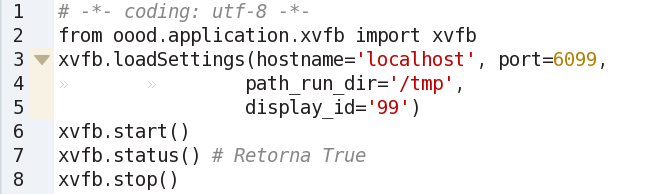
\includegraphics[scale=0.65,bb=0 0 550 156]{xvfb_exemplo.png}
\end{center}
\caption{Utilização da API \textit{IApplication} para controlar o processo Xvfb.}
\label{exemplo:xvfb}
\end{figure}

\begin{figure}[ht]
\centering
\begin{center}
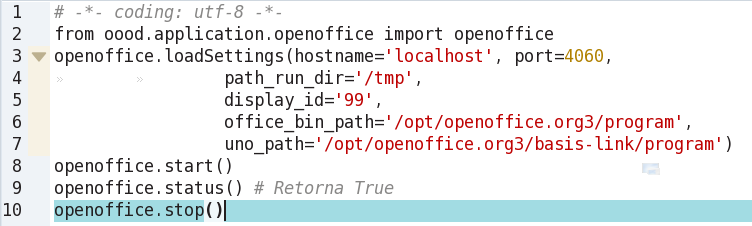
\includegraphics[scale=0.65,bb=0 0 550 156]{openoffice_exemplo.png}
\end{center}
\caption{Utilização da API \textit{IApplication} para controlar o processo OpenOffice.org.}
\label{exemplo:openoffice}
\end{figure}

Nota-se que, na Figura \ref{exemplo:openoffice} existem dois parâmetros de configuração declarados na linha 6 e 7, que não constam na Figura \ref{exemplo:xvfb}. O identificador da interface gráfica, com nome de \textit{display\_id}, em ambos os exemplos são iguais. Essas diferenças de controle entre o processo Xvfb e OpenOffice.org, são justificadas pelo fato de que o OpenOffice precisa do identificador da interface gráfica para iniciar o aplicativo OpenOffice.org e além disso, o caminho do binário do mesmo e da bibliteca UNO.

\section{\textit{IManager}}
\label{obj:manager}

A interface \textit{IManager} é o contrato entre cliente e servidor. Com o objetivo de um contrato mais genérico, foram declarados métodos que futuramente pudessem trabalhar com outros tipos de dados além de documentos. Então, caso a aplicação Web seja estendida para trabalhar, por exemplo, com conversão de vídeos e imagens, o cliente não é afetado.

\subsection{\textit{Manager}}

O classe \textit{Manager} é responsável por criar tarefas enviadas pelo cliente. A Figura \ref{exemplo:manager} apresenta um exemplo da criação de uma tarefa simulando um cliente.

\begin{figure}[ht]
\centering
\begin{center}
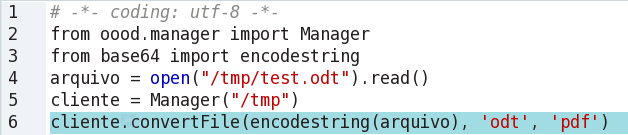
\includegraphics[scale=0.75,bb=0 20 500 85]{manager_exemplo.png}
\end{center}
\caption{Exemplo de utilização do objeto \textit{Manager}.}
\label{exemplo:manager}
\end{figure}

Note que nesta mesma figura, uma biblioteca de codificação é utilizada, chamada \textit{base64}. Esta biblioteca tem como objetivo codificar os dados para transferência pela internet, pois a rede de computadores não suporta o tráfego de documentos em seu estado original.

Como os documentos recebidos pelo objeto \textit{Manager} estão codificados em \textit{base64}, antes de serem salvos no sistema de arquivo, são descodificados para retornar ao estado original. Além disso, os documentos retornados para o usuário também são codificados para serem enviados via rede.

\section{\textit{IDocument}}
No serviço de aplicação OOOD, a prioridade é uma resposta eficiente e consistente ao cliente. Para que isso seja possível é necessário que haja integridade total nos dados enviados para o servidor. Com estes requisitos, a \textit{IDocument} propõe um contrato em que é possível saber o contéudo do documento, atualizá-lo e em casos de problemas em tempo real, recuperar o documento original.

\subsection{\textit{FileSystemDocument}}
\label{fsd}
A classe \textit{FileSystemDocument} utiliza a própria estrutura de pastas do sistema operacional como forma de armazenar os dados. Os arquivos são postos em pastas temporárias que são deletadas quando o objeto não é mais utilizado. Desta forma, cada pasta representa uma requisição do cliente. A Figura \ref{exemplo:fss} demonstra como utilizar este objeto para manipular documentos no sistema de arquivo.

\begin{figure}[!ht]
\centering
\begin{center}
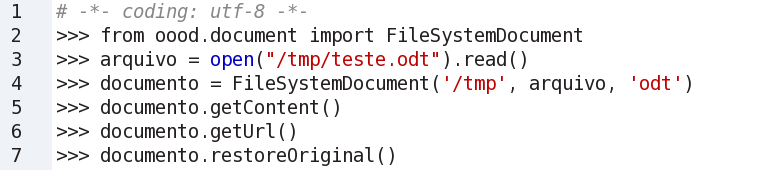
\includegraphics[scale=0.677,bb=0 0 490 95]{fss_exemplo.png}
\end{center}
\caption{Exemplo de uso do \textit{FileSystemDocument}.}
\label{exemplo:fss}
\end{figure}

\section{\textit{IMonitor}}

Com a dificuldade de controle dos processos e os constantes erros que afetavam toda a aplicação, a interface \textit{IMonitor} definiu um contrato que, com atributos mínimos, torna possível monitorar o processo e obter informações à partir disso. Com isso, é possível criar monitores que fiscalizam uma parte da aplicação e caso haja algum resultado não esperado, o pode ser corrigido.

A subseções seguintes apresentam monitores implementados para controlar cada tipo de problema. Portanto, em cada subseção será mostrado o problema e a solução para o mesmo.

\subsection{\textit{MemoryMonitor}}

Com o uso excessivo da conexão entre o OpenOffice.org e o UNO, em muitos casos, a memória utilizada para troca de mensagens não era liberada. Esta falha é a causa de um fenômeno, chamado de vazamento de memória ou \textit{memory leak}, que ocorre em sistemas computacionais quando uma porção de memória alocada para uma determinada operação, não é liberada quando não é mais necessária \cite{1211498}. A consequência disto é o uso de toda memória do computador. 

Para o controle deste problema, a classe \textit{MemoryMonitor} é responsável por fiscalizar a memória utilizada pelo OpenOffice.org e caso esta memória aumente de forma descontrolada o processo é parado imediatamente e reiniciado. Em suma, esta solução foi adicionada pois o sistema operacional não é programado para detectar essas falhas, sendo este erro acusado somente quando toda memória do computador é utilizada.

\subsection{\textit{TimeoutMonitor}}

Com o uso excessivo do OpenOffice.org foi detectado que existem momentos que o mesmo não consegue abrir um documento, pois está travado. Então, a classe \textit{TimeoutMonitor} tem como objetivo limitar o tempo de uso do OpenOffice.org para não permitir que a requisição do cliente fique esperando a resposta por tempo indeterminado. Caso o uso do OpenOffice.org extrapole o tempo máximo, o OpenOffice.org é reiniciado e a requisição é enviada novamente.

\subsection{\textit{RequestMonitor}}

Com o comprometimento da estabilidade do aplicativo à partir de muitas requisições respondidas pelo OpenOffice.org, foi implementado a classe \textit{RequestMonitor}, que reinicia o OpenOffice.org quando o número de requisições respondidas chega ao limite.

\section{\textit{ILockable}}

A exclusão mútua é uma técnica de programação que está inserida em um paradigma de programação chamado de programação concorrente. Esta técnica tem como objetivo impedir que processos ou \textit{threads} tenham acesso a um recurso compartilhado, garantindo a consistência e integridade dos dados \cite{355074}. Este trecho ou recurso compartilhado é chamado de região crítica. Portanto, a interface \textit{ILockable} propõe métodos para controlar a região crítica.

\subsection{OpenOffice}

Além de implementar a interface \textit{IApplication}, descrita na sessão \ref{iapp}, a classe OpenOffice necessita controlar o uso do aplicativo OpenOffice.org, pois este não pode atender mais de uma requisição ao mesmo tempo. Sendo assim, para que haja controle no uso do aplicativo, a classe OpenOffice implementa esta interface, como demonstra a Figura \ref{fig:oo_lockable} o uso de métodos da \textit{ILockable} para controlar o objeto.

\begin{figure}[!ht]
\centering
\begin{center}
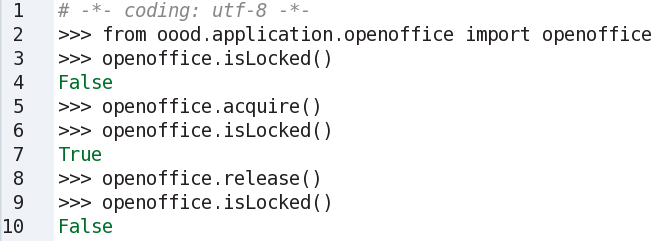
\includegraphics[scale=0.610,bb=0 0 500 146]{open_lockable.png}
\end{center}
\caption{Exemplo de uso da interface \textit{ILockable} no objeto OpenOffice.}
\label{fig:oo_lockable}
\end{figure}

\section{\textit{IHandler}}

Com a necessidade de uma arquitetura flexível, além de fazer com que cada objeto tenha somente uma responsabilidade, foi criada uma interface que é o contrato para objetos responsáveis pela conversão de dados, como por exemplo documentos, vídeos e imagens.

\subsection{\textit{OOHandler}}

A classe \textit{OOHandler} é implementada para comunicar-se com o OpenOffice.org. Quando o serviço OOOD recebe uma requisição, ele automaticamente delega estes dados para o \textit{OOHandler} e requista ao mesmo objeto algum procedimento, por exemplo extrair metadados. Além disso, para armazenar e manusear os dados enviados pelo cliente, o \textit{OOHandler} possui um objeto \textit{FileSystemDocument}, pois caso ocorra falhas, estes dados podem ser restaurados. A Figura \ref{fig:ex_oohandler} demonstra um exemplo de utilização do \textit{OOHandler} e o documento com um objeto \textit{FileSystemDocument}.

\begin{figure}[!ht]
\centering
\begin{center}
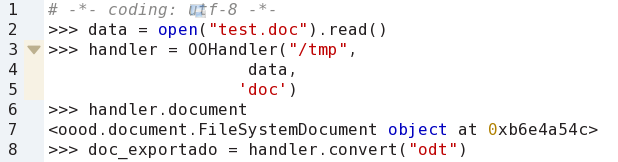
\includegraphics[scale=0.750,bb=0 10 500 106]{ex_oohandler.png}
\end{center}
\caption{Exemplo de utilização do \textit{OOHandler}.}
\label{fig:ex_oohandler}
\end{figure}

\section{\textit{IMimemapper}}

Antes do documento ser aberto pelo OpenOffice.org, existe um pré-processamento para saber o formato do arquivo. Este pré-processamento é necessário, pois para cada extensão existe um filtro específico. 

Em um sistema \textit{desktop} comum, os nomes dos arquivos incluem uma extensão que indica o formato do arquivo, por exemplo ``document.doc''. Antes de abrí-lo na suíte de aplicativos do OpenOffice.org, a suíte detecta a extensão pelo nome do arquivo e através disto abre o arquivo com o filtro referente ao formato. Em casos que o nome do arquivo não define a extensão, o OpenOffice.org tenta descobrir o formato, caso contrário ocorre uma falha dizendo que o arquivo não pode ser aberto pelo aplicativo.

Portanto, com o objetivo de criar um ambiente parecido com um sistema \textit{desktop}, o \textit{IMimemapper} provê métodos para obter todas informações necessárias para manipular um documento antes mesmo de carregá-lo no OpenOffice.org.

\subsection{Filtros do OpenOffice.org}
O aplicativo OpenOffice.org utiliza a linguagem XML para armazenar filtros, extensões e tipos de arquivos. Numa instalação normal, o OpenOffice.org armazena todos esses dados dentro da pasta \textit{TypeDetection} que localiza-se dentro da estrutura de pastas da instalação. Por exemplo, ao utilizar o pacote oficial de instalação, o caminho completo desta pasta seria ``/opt/openoffice.org/basis3.1/share/registry/modules/org/openoffice/TypeDetection''.

Dentro da pasta \textit{TypeDetection} existem duas pastas, que são \textit{Filter} e \textit{Types}. A pasta \textit{Filter} armazena os filtros e o serviço utilizado para exportar um documento utilizando este filtro e \textit{Types} armazena as propriedades de um filtro. As Figuras \ref{fig:type1} e \ref{fig:filter}, demonstram, respectivamente, um exemplo de filtro e tipo declarado no OpenOffice.org. Estes exemplos serão utilizados para explicação dos dados relevantes usados para o Cloudooo.

\begin{figure}[!ht]
\centering
\begin{center}
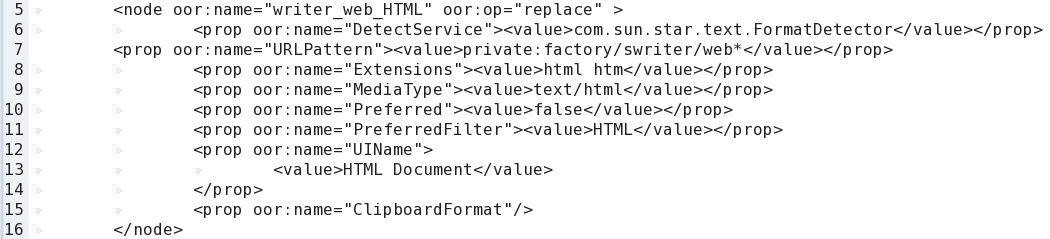
\includegraphics[scale=0.610,bb=0 0 750 166]{type1.jpg}
\end{center}
\caption{Propriedades de um filtro.}
\label{fig:type1}
\end{figure}

\begin{figure}[!ht]
\centering
\begin{center}
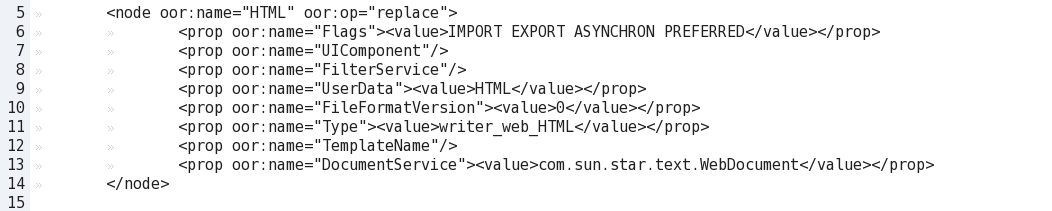
\includegraphics[scale=0.610,bb=0 0 750 146]{filter.jpg}
\end{center}
\caption{Exemplo de um filtro do OpenOffice.org.}
\label{fig:filter}
\end{figure}

Os dados apresentados nas figuras \ref{fig:type} e \ref{fig:filter}, são dados que analisando-os é possível saber qual extensão terá o arquivo caso seja exportado utilizando este filtro. 
\paragraph{}

A ligação entre filtro e tipo é feita pela propriedade \textit{Type} declarado na linha 11 da Figura \ref{fig:filter} e o nome do nó, declarado na linha 5 da Figura \ref{fig:type}. Então, com esta associção, utilizando o filtro HTML o documento terá formato ``htm'' ou ``html'', pois estas extensões estão declarados na propriedade \textit{Extensions}, situado na linha 8 da Figura \ref{fig:type}.
\subsection{\textit{Mimemapper}}
\label{obj:mimemapper}

O UNO possui metódos que possibilitam extrair diversos tipo de informação do OpenOffice.org. A partir disto, a classe \textit{Mimemapper} é responsável por utilizar estes metódos para obter todos os dados necessários para importar e/ou exportar documentos. A Figura \ref{fig:load} apresenta como os filtros são carregados para o \textit{Mimemapper}.

Com os filtros carregados, estes são armazenados em objetos do tipo \textit{Filter}, descrito na sessão \ref{obj:filter}, com o objetivo de tornar fácil o acesso as informações e oferecer uma maior flexibilidade na busca. Por exemplo, na linha 5 da Figura \ref{fig:load}, a partir de informações sobre um determinado formato de arquivo, é possível saber qual nome do filtro é utilizado para importar ou exportar um documento no mesmo formato.

\begin{figure}[!ht]
\centering
\begin{center}
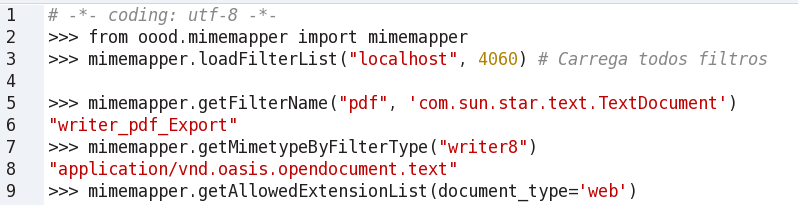
\includegraphics[scale=0.74,bb=0 0 580 140]{mime_load.png}
\end{center}
\caption{Importando todos filtros do OpenOffice.org para o \textit{Mimemapper}.}
\label{fig:load}
\end{figure}


\section{\textit{IFilter}}
\label{interface:filter}

Quando o \textit{Mimemapper}, descrito na sessão \ref{obj:mimemapper}, extrai os filtros do OpenOffice.org, cada um contêm informações que serão utilizadas durante todo o uso da aplicação, mas esses dados precisam ser armanazenados de forma segura e de fácil manuseio. Para isso criou-se um contrato para que cada filtro seja um objeto e tenha métodos que possam extrair suas informações da melhor forma possível.

\subsection{\textit{Filter}}
\label{obj:filter}
O \textit{Filter} é a classe implementada mais simples de toda aplicação. Seu propósito é armazenar todas informações que um filtro do OpenOffice.org possui. A Figura \ref{fig:type} é um exemplo de como criar um filtro e extrair informações do mesmo através do métodos declarados na interface \textit{IFilter}.

\begin{figure}[!ht]
\centering
\begin{center}
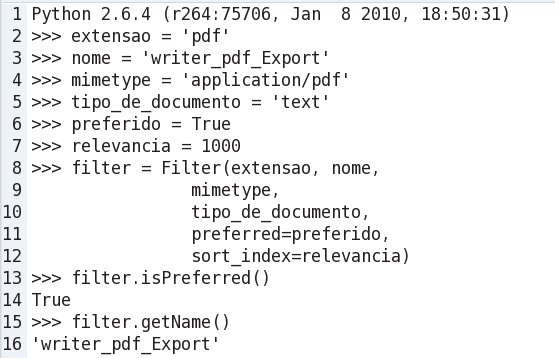
\includegraphics[scale=0.710,bb=0 0 500 250]{exemplo_filter.png}
\end{center}
\caption{Exemplo de criação de um objeto \textit{Filter}.}
\label{fig:type}
\end{figure}
\chapter{Estudo de Casos}
\label{cap5}
Este capítulo apresenta um estudo de caso do Cloudooo e sua implantação no ERP5. O estudo de caso foi idealizado para mostrar a instalação, configuração e uso do Cloudooo no ERP5. Além disso, foi realizado uma comparação entre o Cloudooo e o OOOD.

\section{Ambiente de desenvolvimento}
Para desenvolvimento foi utilizado uma máquina com processador AMD Turion X2 1.6, 2 GB de RAM e 160 GB de HD. O sistema operacional utilizado foi o Mandriva na versão 2010.0, o mesmo que o ERP5 é desenvolvido.

Como pré-requisito de instalação foi necessário ter instalado no sistema operacional o Xvfb e o Python na versão 2.6, pois o OpenOffice.org é instalado junto com a aplicação.

\section{Instalação do Cloudooo}
Para instalação de toda estrutura, é utilizado o Buildout. Este mecanismo de instalação criará um ambiente com todos os pré-requisitos instalados dentro da própria estrutura do Buildout, exceto bibliotecas e aplicativos do sistema operacional. No sistema operacional é necessário que tenha instalado o Xvfb e um Python na versão 2.6 e o pacote \textit{Subversion}.

O procedimento de instalação, após a instalação de todas dependências do sistema operacional, foi fazer download através do repositório SVN \url{https://svn.erp5.org/repos/experimental/oood.buildout}. Este Buildout, foi programado para fazer download do OOOD, que se encontra no repositório SVN \url{http://svn.erp5.org/repos/experimental/oood}. Após isto, acessou-se a pasta que foi criada em seu sistema operacional e executar o arquivo bootstrap.py dentro da pasta bootstrap com o Python 2.6. Com a execução do bootstrap.py, toda estrutura daquela pasta estará ligada diretamente ao python que foi executado. Para ser feita a instalação de todos pacotes necessários e o OpenOffice.org é preciso executar o comando ``bin/buildout'' dentro da mesma pasta.

Na execução deste último comando, além de todas bibliotecas, foi instalado também um OpenOffice.org, versão 3.2, dentro da mesma estrutura. Esta solução foi criada para facilitar a instalação, além de unificar e organizar toda estrutura em um só lugar.

\section{Todos os passos de uma resposta ao cliente}

Para um cliente se conectar ao serviço OOOD, a biblioteca utilizada para comunicação entre o cliente e o servidor é a \textit{xmlrpclib}. A Figura \ref{fig:xmlrpclib.png} demonstra um exemplo de como se conectar ao serviço utilizando a linguagem de programação Python, realizando o envio de uma requisição para o servidor.

\begin{figure}[!ht]
\centering
\begin{center}

\includegraphics[scale=0.660,bb=0 0 600 50]{cliente.png}
\end{center}
\caption{Conexão do cliente com servidor.}
\label{fig:xmlrpclib.png}
\end{figure}

As etapas para conversão de um documento são:
\begin{itemize}
\item O servidor recebe os dados do cliente e estes são inseridos no objeto instanciado \textit{OOHandler};
\item Quando o \textit{OOHandler} recebe os dados, um objeto \textit{FileSystemDocument} é criado para salvar estes dados;
\item Para conversão dos dados, o \textit{OOHandler} bloqueia o objeto OpenOffice para uso, caso este esteja liberado. Caso contrário a requisição espera a liberação do objeto OpenOffice;
\item Quando a conversão do documento é finalizada, o objeto OpenOffice é desbloqueado;
\item Por fim, os dados convertidos são enviados para o cliente e a requisição é toda excluída inclusive os dados armazenados pelo \textit{FileSystemDocument};
\end{itemize}

\section{Instalação do ERP5}
Utilizando o pacote \textit{Subversion}, foi realizado \textit{download} do Buildout para instalação das dependências do ERP5. A Figura \ref{fig:erp5_software} demonstra como fazer \textit{download} do Buildout.

\begin{figure}[!ht]
\centering
\begin{center}

\includegraphics[scale=0.660,bb=0 30 600 20]{erp5_software.png}
\end{center}
\caption{\textit{Download} do Buildout para instalação das dependências do ERP5. Fonte: \cite{erp5_buildout}.}
\label{fig:erp5_software}
\end{figure}

Antes do \textit{download}, foi necessário aceitar um certificado para que os arquivos sejam copiados para a máquina local. Para aceitar este certificado, foi selecionado a opção ``permanente'' para que isto não seja perguntado novamente.

Com os arquivo copiados na máquina local, o próximo passo é instalar todas as dependências através de um \textit{script} que está dentro da pasta ``erp5-software'', criada pelo passo anterior. O comando de execução deste \textit{script} pode ver visto na Figura \ref{fig:dependencies}.

\begin{figure}[!ht]
\centering
\begin{center}

\includegraphics[scale=0.600,bb=0 30 500 20]{erp5_dependencies.png}
\end{center}
\caption{Comando para instalar dependências. Fonte: \cite{erp5_buildout}.}
\label{fig:dependencies}
\end{figure}

Devidamente instaladas todas dependências, o Buildout é executado para instalação dos \textit{softwares}, como por exemplo MySQL, Flare, OOOD. A Figura \ref{fig:make_software} demonstra como executar este comando.

\begin{figure}[!ht]
\centering
\begin{center}

\includegraphics[scale=0.660,bb=0 40 400 65]{make_software.png}
\end{center}
\caption{Comando para instalar configurar o Buildout com as dependências instaladas no sistema operacional. Fonte: \cite{erp5_buildout}.}
\label{fig:make_software}
\end{figure}

Terminada a execução do Buildout, outra estrutura será utilizada para instalação de uma instância do ERP5. Esta separação é aconselhada, pois caso seja necessário criar uma outra instância, já exite um ambiente com todas as dependências instaladas. Então, para instalar a instância, utiliza-se novamente o Buildout, como demonstra a Figura \ref{fig:erp5_data}.

\begin{figure}[!ht]
\centering
\begin{center}

\includegraphics[scale=0.660,bb=50 50 600 70]{erp5_data.png}
\end{center}
\caption{\textit{Download} do Buildout para instalação de uma instância do ERP5. Fonte: \cite{erp5_buildout}.}
\label{fig:erp5_data}
\end{figure}

Novamente após o \textit{download} do Buildout, uma pasta será criada localmente mas com o nome de ``erp5-data''. Nesta pasta são utilizados arquivos de configurações já predefinidos para instalação e configuração da instância do ERP5. Para iniciar a configuração do Buildout foi criado um arquivo com a configuração apresentada na Figura \ref{fig:my_config}, nome ``my\_config.cfg'' e salvo dentro da pasta ``erp5-data''.

\begin{figure}[!ht]
\centering
\begin{center}
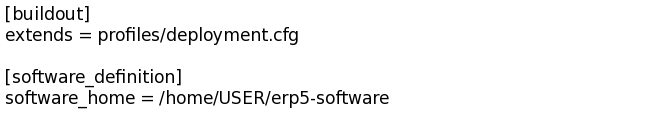
\includegraphics[scale=0.660,bb=0 50 400 120]{erp5_minha_instancia.png}
\end{center}
\caption{Arquivo de configuração ``my\_config.cfg''. Fonte: \cite{erp5_buildout}.}
\label{fig:my_config}
\end{figure}

Note que na Figura \ref{fig:my_config}, possui o nome \textit{USER} no campo ``caminho da pasta''. Este nome deve ser substituido pelo nome do usuário da máquina.

Com este arquivo de configuração, esta instância foi configurada para utilizar todas dependências instaladas no Buildout criado anteriormente. Com isso, não será necessário instalar todos \textit{softwares} novamente, pois esta instância estará utilizando todos recursos do Buildout instalado na pasta ``erp5-software''. A Figura \ref{fig:run_base_instance} apresenta os comandos para configuração desta instância.

\begin{figure}[!ht]
\centering
\begin{center}
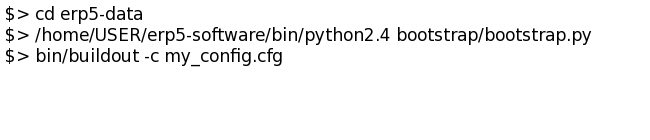
\includegraphics[scale=0.660,bb=0 90 610 120]{run_minha_instancia.png}
\end{center}
\caption{Comandos que configuram as dependências no novo Buildout. Fonte: \cite{erp5_buildout}.}
\label{fig:run_base_instance}
\end{figure}

Após isto, a instância já está configurada com os \textit{softwares}, que serão utilizados pelo ERP5, como por exemplo o OOOD. Com o comando apresentado na Figura \ref{fig:supervisor}, todos estes aplicativos são iniciados.

\begin{figure}[!ht]
\centering
\begin{center}

\includegraphics[scale=0.660,bb=0 30 410 5]{erp5_supervidor.png}
\end{center}
\caption{Comando para iniciar todos aplicativos. Fonte: \cite{erp5_buildout}.}
\label{fig:supervisor}
\end{figure}

Com todas as dependências iniciadas, como por exemplo MySQL e Cloudooo, o próximo passo é a criação da configuração com nome de ``development.cfg'' para criação da instância do ERP5 instalada, desmonstrado na Figura \ref{fig:erp5_site}, e executar o Buildout com este arquivo, apresentado na Figura \ref{fig:run_buildout_again}.

\begin{figure}[ht]
\centering
\begin{center}

\includegraphics[scale=0.660,bb=50 50 410 120]{instancia.png}
\end{center}
\caption{Arquivo de configuração para criação da intância ERP5. Fonte: \cite{erp5_buildout}.}
\label{fig:erp5_site}
\end{figure}

\begin{figure}[ht]
\centering
\begin{center}

\includegraphics[scale=0.660,bb=0 40 410 0]{criar_instancia_erp5.png}
\end{center}
\caption{Comando para criar instância ERP5. Fonte: \cite{erp5_buildout}.}
\label{fig:run_buildout_again}
\end{figure}

Por fim, o comando apresentado na Figura \ref{fig:iniciar_zope} inicia a instância. Como padrão dos arquivos de configuração, a \textit{url} para acessá-la o ERP5 é \url{http://localhost:18080/erp5} com usuário ``zope'' e senha ``zope''.

\begin{figure}[!ht]
\centering
\begin{center}

\includegraphics[scale=0.660,bb=0 50 410 0]{rodar_instancia.png}
\end{center}
\caption{Comando para iniciar instância ERP5. Fonte: \cite{erp5_buildout}.}
\label{fig:iniciar_zope}
\end{figure}

\subsection{Configurando ERP5 para utilizar o Cloudooo}

Após a instalação de toda estrutura do ERP5, foi necessário configurar o OOOD na instância instalada. Acessando a página principal do ERP5, a criação do arquivo de configuração foi realizada pela aba esquerda da mesma página, selecionando a opção ``Preferences'', como mostra a Figura \ref{fig:erp5_click_preferences}. Quando esta opção foi selecionada, a página de preferências do ERP5 foi aberta.

\begin{figure}[!ht]
\centering
\begin{center}
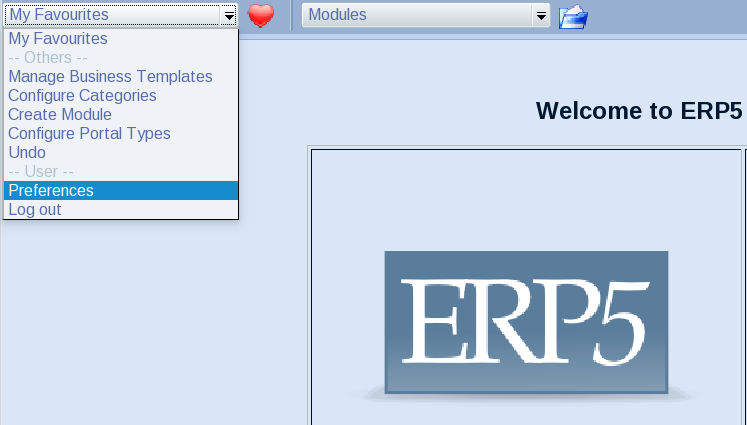
\includegraphics[scale=0.360,bb=0 0 610 290]{erp5_click_preferences.png}
\end{center}
\caption{Opção para acessar as preferências do ERP5.}
\label{fig:erp5_click_preferences}
\end{figure}

Após isto, selecionou-se a aba com nome de ``Action'' na página de prefências e a opção ``Add System Preference'', como demonstra a Figura \ref{fig:action_pref}. Um arquivo de configuração foi criado para que as configurações sejam definidas. A Figura \ref{fig:add_system_pref} apresenta o arquivo de configuração criado.

Com o arquivo de configuração criado, o próximo passo foi definir o endereço do serviço OOOD nos campos ``Conversion Server Address'' para o endereço via internet e ``Conversion Server Port'' para declarar qual porta de acesso na máquina. Por fim, foi salvo as alterações selecionando a ícone igual a um disquete no canto superior direito da página e para utiliza-la, selecionou-se a opção ``Enable Preference'' no campo ``Action''. 

\begin{figure}[!ht]
\centering
\begin{center}
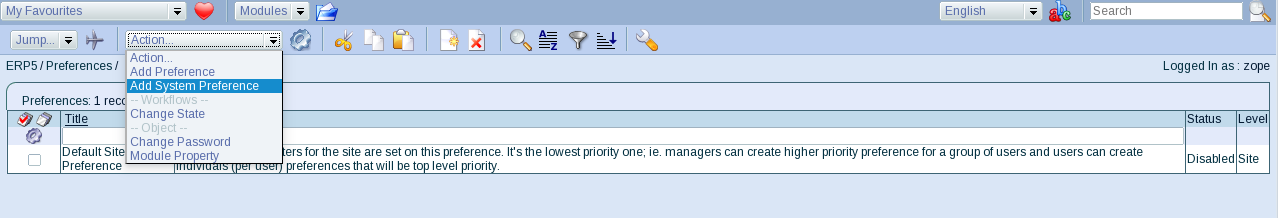
\includegraphics[scale=0.460,bb=0 0 1010 130]{action_pref.png}
\end{center}
\caption{Página de prefêrencias da instância ERP5.}
\label{fig:action_pref}
\end{figure}

\begin{figure}[!ht]
\centering
\begin{center}
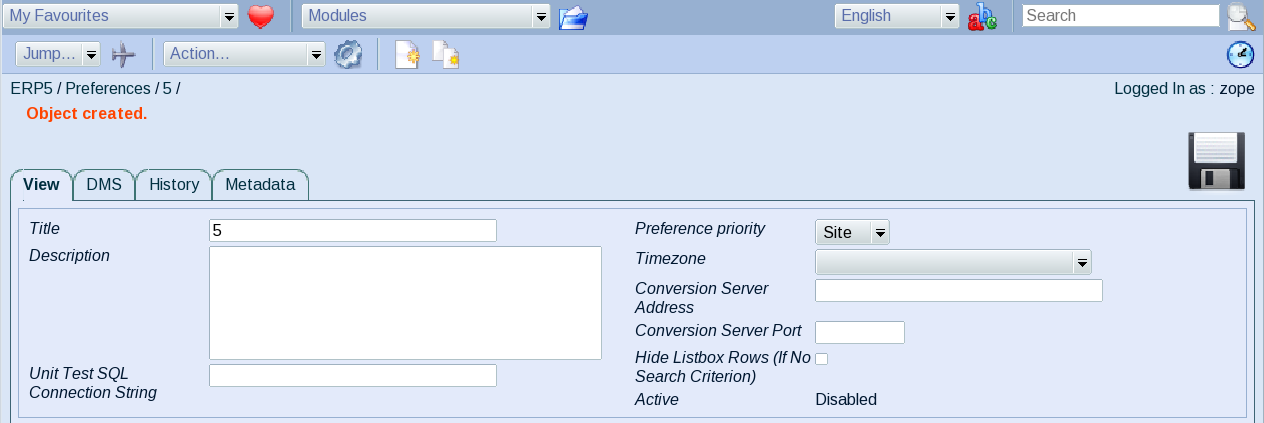
\includegraphics[scale=0.460,bb=0 0 1010 300]{add_system_pref.png}
\end{center}
\caption{Arquivo de configuração da instância.}
\label{fig:add_system_pref}
\end{figure}

\subsection{Instalação do \textit{Business Template} erp5\_dms}

Para que fosse possível inserir documentos no ERP5 foi necessário utilizar o \textit{Business Template}(BT5) erp5\_dms. Para instalação deste pacote acessou-se a principal do ERP e selecionou-se a opção ``Manage Business Templates'' no campo de nome ``My Favourites'', situado no canto esquerdo da mesma página, demonstrado na Figura \ref{fig:manage_bt5}.

\begin{figure}[!ht]
\centering
\begin{center}
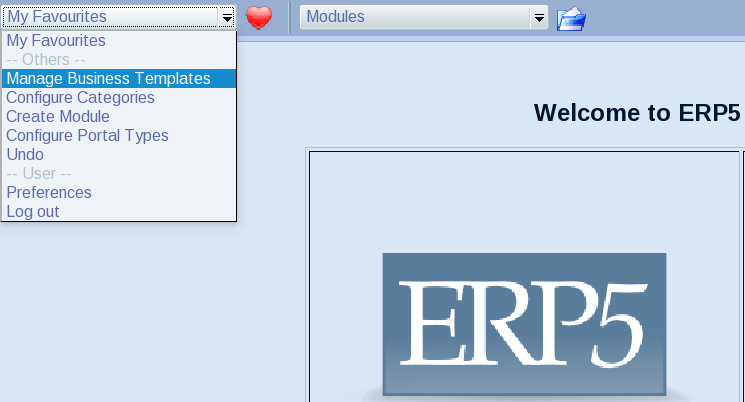
\includegraphics[scale=0.430,bb=0 45 610 257]{manage_bt5.png}
\end{center}
\caption{Opção para acessar a página de configuração dos \textit{Business Templates}.}
\label{fig:manage_bt5}
\end{figure}

Após isto, foi selecionado o botão ``Import \ Export'', indicado pela seta na Figura \ref{fig:import_export.png}, para que a página de atualização dos \textit{Business Templates} fosse aberta. No campo "Repositories" definiu-se o repositório \url{http://www.erp5.org/dists/snapshot/bt5}. A Figura \ref{fig:update_bt5.png} demonstra a página de atualização e o campo a ser preenchido.

\begin{figure}[!ht]
\centering
\begin{center}
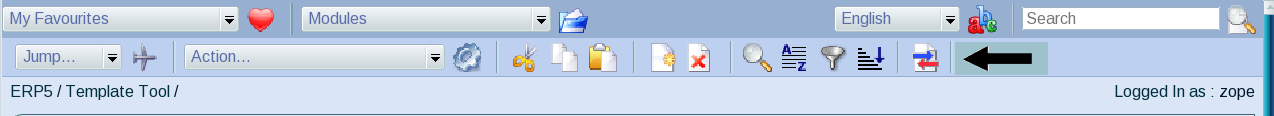
\includegraphics[scale=0.490,bb=0 30 1010 70]{import_export.png}
\end{center}
\caption{Botão para importar ou exportar \textit{Business Templates}.}
\label{fig:import_export.png}
\end{figure}

\begin{figure}[!ht]
\centering
\begin{center}
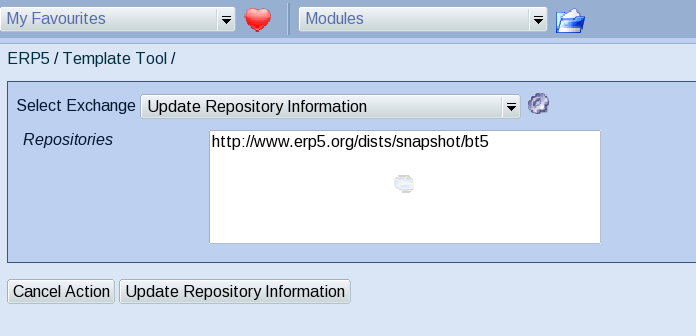
\includegraphics[scale=0.490,bb=0 30 510 210]{update_bt5.png}
\end{center}
\caption{Página para definir o endereço do repositório a ser utilizado.}
\label{fig:update_bt5.png}
\end{figure}

Definindo o repositório a ser utilizado, clicou-se em ``Update Repository Information'' para salvar a \textit{url} adicionada e, após isto, selecionou-se a opção ``Install Business Templates from Repositories'' no campo ``Select Exchange'' para que a lista de BT5 fosse exibida como demonstra a Figura \ref{fig:lista_bt5.png}.

\begin{figure}[!ht]
\centering
\begin{center}
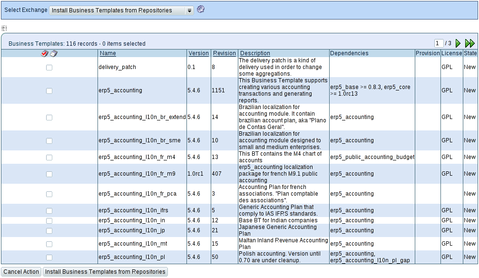
\includegraphics[scale=0.620,bb=0 30 410 190]{lista_erp5.png}
\end{center}
\caption{Lista de \textit{Business Templates} instaláveis. Fonte: \cite{erp5_bt5}.}
\label{fig:lista_bt5.png}
\end{figure}

Na página de listagem dos \textit{Business Templates}, selecionou-se os seguintes pacotes para instalação do erp5\_dms:
\begin{itemize}
 \item erp5\_base
 \item erp5\_dms;
 \item erp5\_web;
 \item erp5\_ingestion;
 \item erp5\_ingestion\_mysql\_innodb\_catalog;
\end{itemize}

Feito a seleção dos pacotes, clicou-se em ``Install Business Templates from Repositories'' no final da página e uma janela de validação de todos arquivos instaladaos foi exibida, como demonstra a Figura \ref{fig:validate_packages}. Para validar a instalação clicou-se em ``Validate Installation'' para que todos os pacotes fosse instalados.

\begin{figure}[!ht]
\centering
\begin{center}
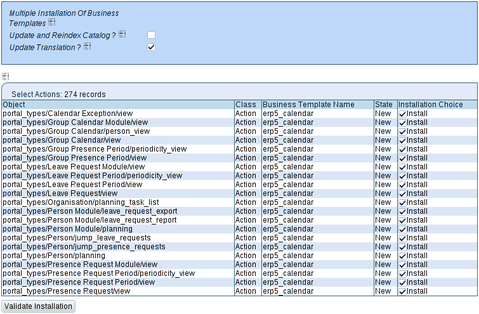
\includegraphics[scale=0.620,bb=0 30 390 210]{validate_packages.png}
\end{center}
\caption{Lista de \textit{Business Templates} instaláveis. Fonte: \cite{erp5_bt5}.}
\label{fig:validate_packages}
\end{figure}

\section{Compatibilidade entre o ERP5 e o Cloudooo}

Como o ERP5 possui muitos ambientes em produção, o custo para migrar todos estes ambientes para uma nova API seria muito grande. De tal forma, foi implementado uma interface de compatibilidade entre a aplicação Web e o ERP para redução de custo de migração para a nova API. Com isso, haverá a diminuição de falhas em ambientes de produção. Por exemplo, o metódo apresentado na Figura \ref{fig:run_convert} recebe os parâmetros da mesma forma que são enviados pelo ERP5, chama o metódo da nova API e retorna os dados como é esperado pelo ERP5.

\begin{figure}[!ht]
\centering
\begin{center}
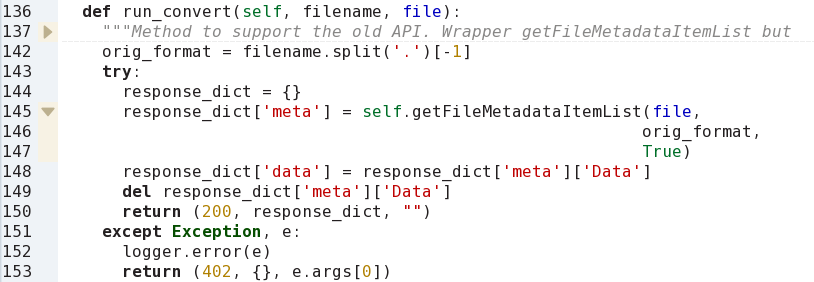
\includegraphics[scale=0.660,bb=0 0 600 190]{run_convert.png}
\end{center}
\caption{Trecho de código que representa um dos métodos de compatibilidade entre aplicações.}
\label{fig:run_convert}
\end{figure}

\section{Usando o ERP5 para converter documentos}

O OOOD é utilizado dentro do ERP5 para converter e extrair metadados de documentos. Para enviar um documento para o ERP5 clicou-se no \textit{link} ``Documents'' na página principal do ERP, como demonstra a Figura \ref{fig:erp5_click_documents}.

\begin{figure}[!ht]
\centering
\begin{center}
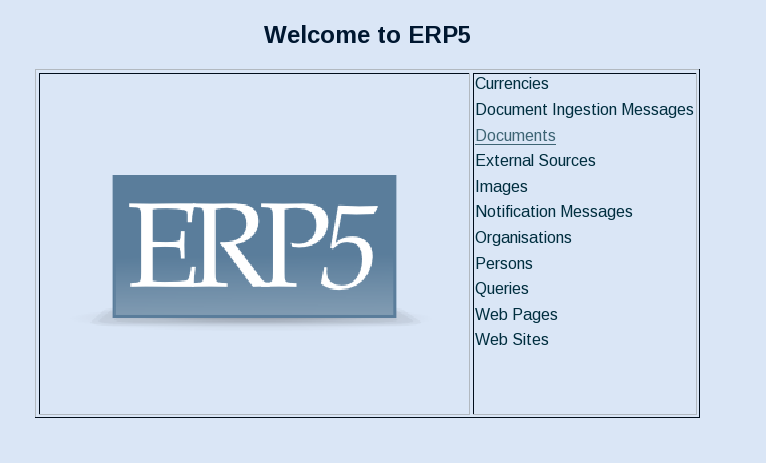
\includegraphics[scale=0.400,bb=0 40 600 310]{erp5_click_documents.png}
\end{center}
\caption{Página Principal do ERP5.}
\label{fig:erp5_click_documents}
\end{figure}

Após isto, na aba ``Action'' selecionou-se a opção ``Add Text'', demonstrado na Figura \ref{fig:add_text}. Na página seguinte foi inserido o documento e o nome para este, como mostra a Figura \ref{fig:upload_text}. Note que nesta mesma figura, quando o arquivo foi inserido e salvo, o estado deste arquivo é alterado de ``Empty'', depois para ``Converting'' e por fim ``Converted''. Isto significa que o documento foi enviado para extrair os metados e convertido para a base ODF.

\begin{figure}[!ht]
\centering
\begin{center}
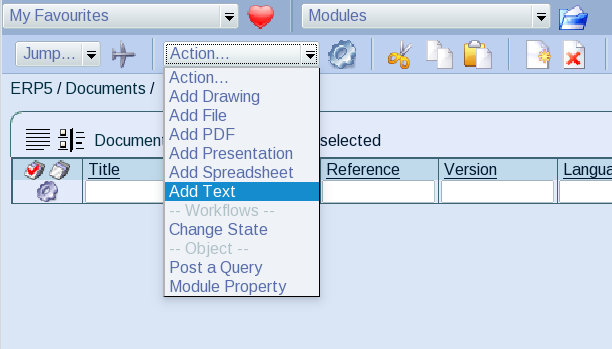
\includegraphics[scale=0.570,bb=0 30 510 240]{add_text.png}
\end{center}
\caption{Opção para criar um objeto documento no ERP5.}
\label{fig:add_text}
\end{figure}

\begin{figure}[!ht]
\centering
\begin{center}
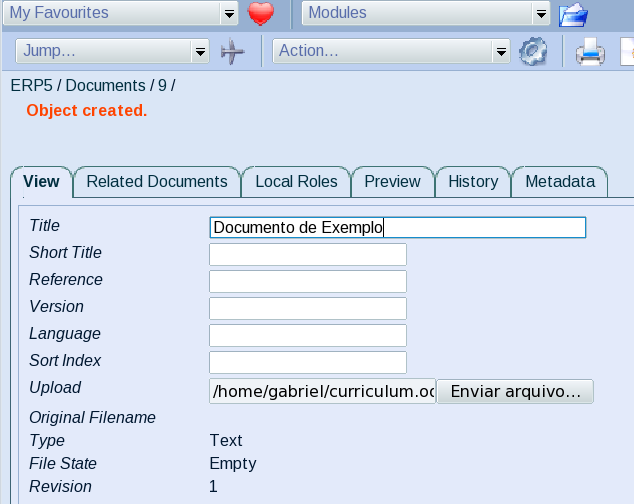
\includegraphics[scale=0.570,bb=0 30 510 340]{upload_text.png}
\end{center}
\caption{\textit{Upload} de um documento.}
\label{fig:upload_text}
\end{figure}

Para este documento ser vizualizado através do ERP5, clicou-se na aba ``Preview'', como demonstra a Figura \ref{fig:preview_erp5}. Quando a opção de vizualização foi selecionada, o documento foi convertido para o formato html para que seja possível vizualizá-lo no ERP.

\begin{figure}[!ht]
\centering
\begin{center}
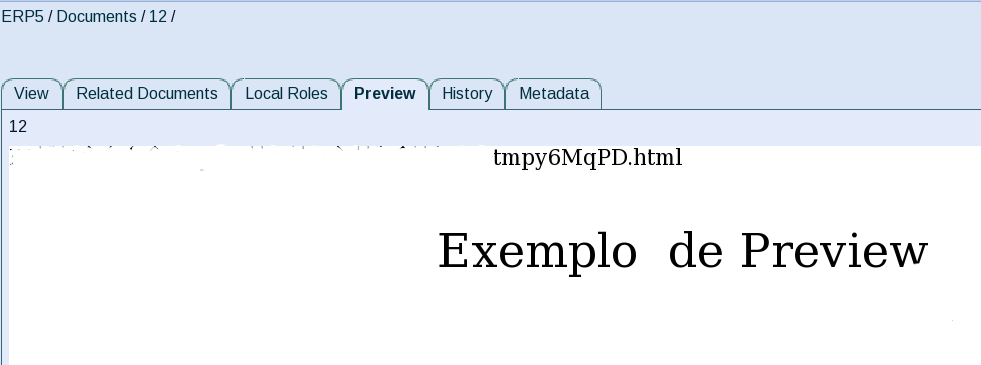
\includegraphics[scale=0.570,bb=0 30 810 240]{preview_erp5.png}
\end{center}
\caption{Pré-visualização de um documento.}
\label{fig:preview_erp5}
\end{figure}

Além disso, em documentos em formatos para apresentação é possível através da aba \textit{Preview} fazer \textit{download} do documento completo no formato pdf. Para isto, clicou-se em ``Download as PDF'' no final da página de pré-vizualização.

\section{Problemas e Decisões de Projeto}

Com o desenvolvimento e testes excessivos na aplicação, algumas decisões de projeto foram tomadas para obter resultados mais eficientes ao clientes e correção de erros graves. Nesta sessão é explicado decisões que, em alguns casos, mudaram a arquitetura do projeto.

\subsection{Vazamento de memória}

O uso excessivo da aplicação OOOD mostrou que em algumas conexões entre o UNO e o OpenOffice.org, a memória utilizada não era completamente liberada. Este aumento gradativo do uso da memória, ocasiona um erro no sistema operacional, chamado \textit{memory leak}, que ocorre quando não há mais memória livre para ser utilizada. 

Com os resultados dos testes e a análise do uso de memória, foi possível detectar que o erro está no UNO que não libera a memória corretamente quando a conexão com o OpenOffice.org termina. Além disso, foi detectado também que a memória somente é liberada corretamente quando todo o processo é finalizado, ou seja, quando o serviço é parado. Para que isso fosse resolvido foi necessário remover a biblioteca UNO da memória quando esta não estivesse sendo utilizada.

A solução para este problema foi a implementação de dois \textit{scripts} que fazem toda comunicação entre o OOOD e o OpenOffice.org. Desta forma, quando os \textit{scripts} terminarem os procedimentos, toda memória utilizada será liberada e o serviço não sofrerá alteração, caso ocorram falhas.

Estes \textit{scripts} foram implementados com objetivos diferentes, logo, as sessões abaixo explicam cada \textit{script} e seus objetivos.

\subsubsection{UnoConverter}

O \textit{script UnoConverter} foi implementado para conter as mesmas funcionalidades que o \textit{OOHandler}. Esta implementação tem como objetivo retirar a comunicação entre OOOD e o OpenOffice.org. Com isso, o \textit{OOHandler} utiliza o \textit{script UnoConverter} para se comunicar com o OpenOffice.org.

Desta forma, a memória utilizada pela comunicação entre o \textit{script UnoConverter} e o OpenOffice.org é liberada assim que o \textit{script} é finalizado.

\subsubsection{UnoMimeMapper}

Além do acesso constante para conversão de documentos, uma outra necessidade de acesso ao OpenOffice.org é a extração de filtros feito pelo \textit{MimeMapper}. Como este é um componente da aplicação OOOD, o \textit{UnoMimeMapper} é utilizado para extrair os filtros do OpenOffice.org e retorná-los para o \textit{MimeMapper}.

\subsection{Armazenamento e busca dos filtros}

A partir da extensão de um documento, como por exemplo ``doc'', é possível saber para quais formatos este documento pode ser exportado. Com o objetivo de fazer com que esta funcionalidade tenha um desempenho melhor, foram criadas três estruturas que armazenam as informações de maneiras diferentes para minimizar o tempo de busca pelos dados. As três maneiras são:

\begin{itemize}
\item Filtro por Extensão - armazena os filtros a partir da extensão do arquivo. Utilizada para selecionar o filtro adequado para exportar o documento;

\item Extensões por Tipo de documento - armazena extensões de acordo com o seu tipo. Utilizado para buscar extensões de acordo com o tipo do documento;

\item Tipo de Documento por extensão - armazena os tipos dos documentos suportados pela extensão. Com esta estrutura é possível verificar se a extensão de destino do documento suporta o mesmo tipo que a extensão do arquivo original;
\end{itemize}

Em suma, durante a importação dos filtros, os dados extraídos são organizados para eliminar qualquer processamento na hora de buscar por informações.

\subsection{Arquivos compactados}

Arquivos no formato ``html'' e ``htm'' não suportam imagens dentro do corpo do arquivo. Para que a imagem seja visualizada junto com o conteúdo em páginas Web, o caminho da imagem é inserido dentro código do documento. Como a aplicação OOOD suporta conversões de documentos, tanto o arquivo enviado ou recebido pelo o cliente em formatos ``html'' ou ``htm'', é necessário que as imagens sejam enviadas junto com o documento, caso contrário o documento gerado será inválido. Para que isto seja possível, o \textit{FileSystemDocument} suporta compactação e descompactação de arquivos.

O caso de descompactação ocorre quando o cliente envia um arquivo e este está compactado. Neste caso, todos os dados são extraídos, salvos na mesma pasta, o arquivo original é removido e o arquivo com nome \textit{index.html} é posto como documento principal.

Em contrapartida, a compactação é requisitada pelo usuário e, caso seja, o \textit{FileSystemDocument} compacta todos arquivos que estão dentro da pasta e envia para o cliente.

\section{Explicando o funcionamento do prestador de serviço com \textit{Paste}}

Para provêr os serviços do OOOD, foi utilizado a ferramenta \textit{Paste}, que é um conjunto de ferramentas para construção de aplicativos e, além disso, provê serviços que implementam a interface WSGI.

Para configurar a aplicação OOOD com o \textit{Paste}, foi definido no arquivo \textit{setup.py} da aplicação, qual metódo seria utilizado para iniciar o serviço, como demonstra a Figura \ref{fig:setup}.

Com a definição apresentada pela Figura \ref{fig:setup}, o método de nome \textit{application} será responsável por iniciar o serviço. Além disso, este mesmo método, de acordo com o WSGI, deve retornar no final de seu procedimento qual método o cliente recebe ao se conectar com o serviço.

\begin{figure}[!ht]
\centering
\begin{center}
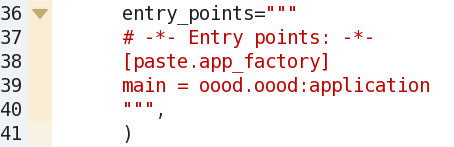
\includegraphics[scale=0.620,bb=0 30 310 100]{setup_py_paste.png}
\end{center}
\caption{Definição do metódo que irá prover o serviço.}
\label{fig:setup}
\end{figure}

\begin{figure}[!ht]
\centering
\begin{center}
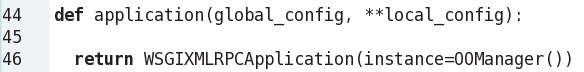
\includegraphics[scale=0.620,bb=0 30 510 60]{oood_application.png}
\end{center}
\caption{Método que inicia a aplicação e retorno do objeto que o cliente recebe quando se conecta.}
\label{fig:application}
\end{figure}

Por fim, para iniciar uma aplicação utilizando a ferramenta \textit{Paste}, esta última necessita de um arquivo de configuração que possui informações como, o pacote do \textit{Paste} a ser utilizado e a porta que o servidor deve ser iniciado. A Figura \ref{fig:oood_conf} demonstra um trecho do arquivo de configuração para iniciar a aplicação OOOD e a Figura \ref{fig:start_paste} demonstra como a aplicação é iniciada utilizando esta aplicação.

\begin{figure}[!ht]
\centering
\begin{center}
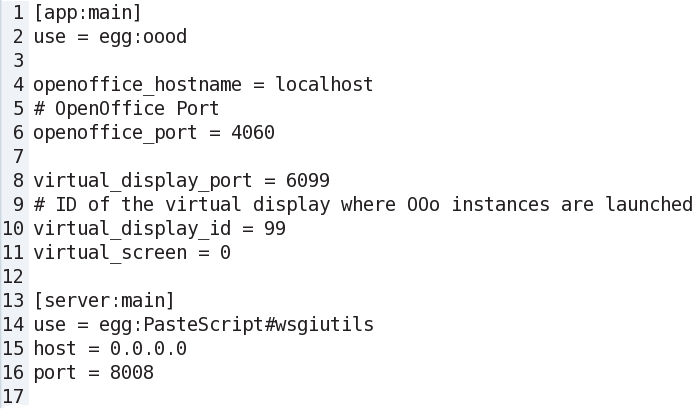
\includegraphics[scale=0.520,bb=0 30 510 280]{oood_conf.png}
\end{center}
\caption{Amostra do arquivo de configuração.}
\label{fig:oood_conf}
\end{figure}

\begin{figure}[!ht]
\centering
\begin{center}

\includegraphics[scale=0.570,bb=0 30 510 0]{start_paste.png}
\end{center}
\caption{Iniciando a aplicação OOOD com \textit{Paste}.}
\label{fig:start_paste}
\end{figure}

\section{Comparando a \textit{perfomance} entre a Cloudooo e o OOOD}

Para comparar melhor o desenvolvimento da nova aplicação, foram desenvolvidos \textit{scripts} que submetiam documentos tanto para nova aplicação quanto para a antiga. Nestes scripts, foram registrados o tempo de conversão de cada documento e o tempo total de todas as conversões.

Para realização destes testes foram selecionados 3699 documentos no formato odt, sendo alguns destes inválidos e outros em formatos desconhecidos. Além disso, para realização destes testes foi definido que o formato destino dos documentos fosse o pdf, pois este formato é o mais utilizado pelo ERP5 para exportar documentos.

Com o resultado dos testes, notou-se que a conversão do primeiro documento é mais rápida no OOOD. Mas, com o uso excessivo das aplicações e com os erros gerados, o Cloudooo se manteve estável enquanto o OOOD apresentou-se instável em relação ao tempo de conversão. Os erros apresentados pelo Cloudooo foram 12 de arquivos inválidos, enquanto a aplicação antiga apresentou 531 erros.

Apesar do Cloudooo individualmente ser mais lento para arquivos individuais, o tempo gasto para conversão de todos foi de 10 horas. Enquanto a aplicação antiga gastou 11 horas para finalizar as conversões.

\section{Resultados obtidos}

No estudo de caso foi apresentado a utilização da aplicação OOOD junto com a ferramenta \textit{Paste}, que provê o serviço. Além disso, foi  instalado e configurado o ERP5 e o \textit{Business Templates} para conversão e extração de metadados de documentos utilizando o OOOD.

Vale ressaltar que, a ferramenta que provê o serviço utilizada neste estudo de caso, pode ser substituída por qualquer outra ferramenta que forneça serviços que utilizem o padrão WSGI. Isto demonstra que o serviço pode ser modificado de acordo com a necessidade e demanda dos clientes.

Além disso, foram apresentados dados comprovando que com a utilização de uma arquitetura mais atual e flexível, trouxeram resultados satisfátorios.

\chapter{Conclusão}
\label{conclusao}
\section{Objetivos alcançados}
Neste trabalho foi apresentado o \textit{Web Service} OOOD 2.0, uma ferramenta \textit{Open Source} para conversão de documentos em larga escala. Sua implementação de forma genérica, fez com que cada parte da aplicação possa ser utilizada separamente como uma biblioteca comum, tornando possível adicionar uma nova implementação caso almeje-se extender para atender requisitos específicos.

Foi visto também que, com o Python e seus recursos, é possível desenvolver ferramentas que suportam grandes demandas sem que a legibilidade e flexibilidade do código sejam esquecidas.

\section{Trabalhos futuros}

Implementar manipuladores de imagens e vídeos para que seja possível converter e extrair metadados destes tipos de arquivos. Além disso, diminuir os dados que são tranferidos entre os componentes da aplicação e os \textit{scripts} \textit{UnoConverter} e \textit{UnoMimeMapper} pois, diminuindo o tamanho dos dados, há um redução direta no tempo de resposta para o cliente.

É necessário também melhorar o ambiente de testes para que não seja necessário iniciar e parar o OpenOffice.org a cada teste, ou seja, para que os testes executem iniciando e parando o OpenOffice.org somente um vez, diminuindo o tempo gasto para executá-los.
\end{spacing}

\begin{spacing}{1.5}
\bibliographystyle{abnt-alf}
\bibliography{referencia}
\end{spacing}

\begin{spacing}{1.5}
\include{apendice}
\end{spacing}

\end{document}
